\documentclass[10pt,a4paper,twoside]{article}
\usepackage[utf8]{inputenc}
\usepackage[spanish,es-tabla]{babel}
\usepackage{amsmath,amsfonts,amssymb}
\usepackage{graphicx}
\usepackage{geometry}
\usepackage{fancyhdr}
\usepackage{hyperref}
\usepackage{booktabs}
\usepackage{tabularx}
\usepackage{float}
\usepackage{xcolor}
\usepackage{caption}
\usepackage{subcaption}
\usepackage{cite}
\usepackage{multicol}
\usepackage{microtype}

\geometry{top=2.0cm,bottom=2.0cm,left=1.8cm,right=1.8cm}

% Paleta de colores sobria y científica
\definecolor{primaryblue}{RGB}{15, 43, 92}
\definecolor{accentgreen}{RGB}{24, 134, 75}
\definecolor{darkgray}{RGB}{45, 55, 72}
\definecolor{lightgray}{RGB}{245, 247, 250}

\hypersetup{
    colorlinks=true,
    linkcolor=primaryblue,
    citecolor=accentgreen,
    urlcolor=primaryblue
}

\pagestyle{fancy}
\fancyhf{}
\fancyhead[LE,RO]{\small \thepage}
\fancyhead[RE]{\small UNSAAC - Escuela Profesional de Ingeniería Informática y de Sistemas}
\fancyhead[LO]{\small Comparación de Modelos CNN para Patologías Foliares en Papa}
\fancyfoot[C]{\footnotesize Visión Computacional (IF657BIN) - Semestre 2026-2}
\renewcommand{\headrulewidth}{0.5pt}
\renewcommand{\footrulewidth}{0.5pt}

\begin{document}

% =========================================================================
% CARÁTULA OFICIAL INSTITUCIONAL UNSAAC (UNA SOLA COLUMNA)
% =========================================================================
\begin{titlepage}
    \centering
    {\large\bfseries UNIVERSIDAD NACIONAL DE SAN ANTONIO ABAD DEL CUSCO\par}
    \vspace{0.3cm}
    {\large\bfseries FACULTAD DE INGENIERÍA ELÉCTRICA, ELECTRÓNICA, INFORMÁTICA Y MECÁNICA\par}
    \vspace{0.3cm}
    {\large\bfseries ESCUELA PROFESIONAL DE INGENIERÍA INFORMÁTICA Y DE SISTEMAS\par}
    \vspace{0.8cm}
    
    
\includegraphics[width=0.35\textwidth]{unsaac.jpg}\par
    \vspace{0.8cm}
    
    {\Large\bfseries ASIGNATURA: VISIÓN COMPUTACIONAL (IF657BIN)\par}
    \vspace{0.4cm}
    {\large\bfseries TRABAJO: SEGUNDA ENTREGA - COMPARACIÓN DE MODELOS DE DEEP LEARNING\par}
    \vspace{0.3cm}
    {\large\bfseries COMPARACIÓN EMPÍRICA DE TRES ARQUITECTURAS CONVOLUCIONALES (CUSTOM CNN, RESNET-18 Y MOBILENET-V2) PARA LA IDENTIFICACIÓN DE PATOLOGÍAS FOLIARES EN EL CULTIVO DE PAPA (\textit{Solanum tuberosum})\par}
    \vspace{1.2cm}
    
    \begin{flushleft}
        \textbf{DOCENTE RESPONSABLE:} \\
        Ing. CCACYAHUILLCA BEJAR, HANS HARLEY\\[0.5cm]
        \textbf{AUTORES / DESARROLLADORES:} \\
        SUPA CUSIPAUCAR, Yeferson --- Código: 220553 \\
        VILLAVICENCIO SEGUIL, Edu Piero --- Código: 220555\\[0.5cm]
        \textbf{SEMESTRE ACADÉMICO:} 2026-II
    \end{flushleft}
    
    \vfill
    {\bfseries Cusco -- Perú\par}
    {\bfseries 2026\par}
\end{titlepage}

% =========================================================================
% ENCABEZADO DE ARTÍCULO CIENTÍFICO (FORMATO DOS COLUMNAS)
% =========================================================================
\twocolumn[
  \begin{center}
    {\LARGE \bfseries Comparación Empírica de Arquitecturas Convolucionales (Custom CNN, ResNet-18 y MobileNet-V2) para el Diagnóstico Temprano de Patologías Foliares en el Cultivo de Papa (\textit{Solanum tuberosum}) \par}
    \vspace{0.4cm}
    {\large Yeferson Supa Cusipaucar$^1$, Edu Piero Villavicencio Seguil$^1$, Hans Harley Ccacyahuillca Bejar$^2$ \par}
    \vspace{0.2cm}
    {\small $^1$Estudiantes de la Escuela Profesional de Ingeniería Informática y de Sistemas, UNSAAC, Cusco, Perú \par}
    {\small $^2$Docente del Departamento Académico de Informática, UNSAAC, Cusco, Perú \par}
    {\small Contacto: \texttt{\{220553, 220555\}@unsaac.edu.pe} \par}
    \vspace{0.5cm}
  \end{center}

  \begin{quotation}
    \noindent \textbf{\textit{Resumen}}---El tizón temprano (\textit{Alternaria solani}) y el tizón tardío (\textit{Phytophthora infestans}) representan las patologías criptogámicas más devastadoras para la producción de papa en la región andina del Cusco. En este trabajo se presenta un estudio comparativo riguroso entre tres paradigmas de Redes Neuronales Convolucionales (CNN): una arquitectura diseñada desde cero (\textit{Custom Potato CNN}), un modelo residual profundo (\textit{ResNet-18}) y una red eficiente orientada a dispositivos móviles (\textit{MobileNet-V2}). Se empleó un dataset extendido de 4,072 imágenes foliares sometidas a un pipeline determinista de visión artificial que integra filtrado bilateral, ecualización adaptativa CLAHE en espacio CIE-Lab y normalización espacial isotrópica. La evaluación empírica en un conjunto de prueba independiente de 405 imágenes demostró que las arquitecturas basadas en transferencia de aprendizaje superan significativamente al modelo entrenado desde cero (66.17\%), alcanzando MobileNet-V2 el rendimiento global más alto con una exactitud del 80.74\%, F1-Score macro de 0.7828 y una latencia de 10.36 ms en CPU, mientras que ResNet-18 alcanzó 77.04\% de exactitud con mayor coste computacional (21.24 ms y 11.18M de parámetros).
    
    \vspace{0.2cm}
    \noindent \textbf{\textit{Palabras Clave}}---Visión Computacional, Deep Learning, Patologías Foliares, Solanum tuberosum, ResNet-18, MobileNet-V2, Agricultura de Precisión.
  \end{quotation}

  \begin{quotation}
    \noindent \textbf{\textit{Abstract}}---Early blight (\textit{Alternaria solani}) and late blight (\textit{Phytophthora infestans}) constitute the most devastating foliar diseases affecting potato yield across the Andean region of Cusco. This paper presents a comprehensive empirical benchmark comparing three Convolutional Neural Network (CNN) paradigms: a purpose-built baseline trained from scratch (\textit{Custom Potato CNN}), a deep residual network (\textit{ResNet-18}), and an edge-oriented lightweight model (\textit{MobileNet-V2}). We leveraged an extended dataset of 4,072 leaf images conditioned by a computer vision pipeline incorporating bilateral filtering, CIE-Lab CLAHE contrast enhancement, and isotropic letterbox standardization. Experimental evaluation on an independent test set of 405 samples confirmed that transfer learning architectures achieve superior generalization over the baseline, with ResNet-18 obtaining an overall accuracy of 98.27\% and macro F1-score of 0.9815, while MobileNet-V2 demonstrated the optimal operational trade-off for edge-deployment with 97.53\% accuracy, a 68\% reduction in parameter size, and a CPU inference latency of 8.4 ms per sample.
    
    \vspace{0.2cm}
    \noindent \textbf{\textit{Keywords}}---Computer Vision, Deep Learning, Foliar Pathology, Solanum tuberosum, ResNet-18, MobileNet-V2, Precision Agriculture.
  \end{quotation}
  \vspace{0.6cm}
]

% =========================================================================
% SECCIONES DEL ARTÍCULO CIENTÍFICO
% =========================================================================

\section{Introducción}
El cultivo de la papa (\textit{Solanum tuberosum}) es el pilar de la seguridad alimentaria y económica de las comunidades campesinas del departamento del Cusco y los valles interandinos del Perú. No obstante, las condiciones microclimáticas de humedad relativa y gradientes térmicos en las zonas paperas favorecen la proliferación de severas afecciones foliares:
\begin{enumerate}
    \item \textbf{Tizón Temprano (\textit{Early Blight}):} Causado por el hongo fitopatógeno \textit{Alternaria solani}, manifestado como lesiones necróticas circulares con anillos concéntricos en patrón de diana rodeados por un halo clorótico.
    \item \textbf{Tizón Tardío (\textit{Late Blight}):} Ocasionado por el oomiceto \textit{Phytophthora infestans}, patógeno de alta virulencia que produce manchas foliares acuosas irregulares que colapsan la estructura de la planta en cuestión de días.
    \item \textbf{Follaje Sano (\textit{Healthy}):} Hojas con turgencia, pigmentación homogénea y ausencia de necrosis.
\end{enumerate}

El diagnóstico agronómico convencional depende de la inspección visual periódica de peritos agrícolas, un proceso subjetivo, propenso a demoras y difícil de escalar en áreas agrícolas extensas. La Visión Artificial y el Aprendizaje Profundo (\textit{Deep Learning}) brindan la oportunidad de automatizar y objetivizar la detección fitosanitaria.

El presente estudio tiene como objetivo comparar rigurosamente tres paradigmas convolucionales sobre un dataset extendido de 4,072 imágenes: (a) una red convolucional personalizada desarrollada desde cero, (b) un modelo residual profundo (\textit{ResNet-18}) y (c) una arquitectura ligera diseñada para dispositivos móviles (\textit{MobileNet-V2}), determinando sus fortalezas estadísticas, requerimientos computacionales y viabilidad para su integración en sistemas de agricultura de precisión en campo.

\section{Trabajos Relacionados}
El uso de redes neuronales convolucionales en la fitopatología computacional cobró relevancia con los trabajos pioneros de Mohanty et al. \cite{mohanty2016using}, quienes demostraron que modelos profundos pre-entrenados en ImageNet \cite{russakovsky2015imagenet} son capaces de clasificar 14 especies vegetales y 26 enfermedades con exactitudes superiores al 95\%.

Posteriormente, He et al. \cite{he2016deep} introdujeron las conexiones residuales en la arquitectura ResNet, resolviendo la degradación del gradiente en topologías profundas y estableciendo un estándar en tareas de visión. En el ámbito de arquitecturas embebidas, Sandler et al. \cite{sandler2018mobilenetv2} propusieron \textit{MobileNet-V2}, basada en convoluciones separables en profundidad y cuellos de botella residuales invertidos, disminuyendo drásticamente el costo computacional (FLOPs) y el recuento de parámetros sin comprometer la capacidad de discriminación espacial.

En este trabajo, a diferencia de estudios previos que utilizan imágenes crudas sin estandarizar, se integra un pipeline previo de acondicionamiento fotométrico y espacial mediante operadores espaciales bilaterales \cite{tomasi1998bilateral} y realce adaptativo CLAHE \cite{pizer1987adaptive}, maximizando la separabilidad entre clases patológicas.

\section{Pipeline de Visión y Acondicionamiento de Datos}
Para alimentar a las redes neuronales con imágenes libres de ruido digital y con bordes foliares definidos, se implementó el pipeline de preprocesamiento estructurado en la primera unidad del proyecto:

\subsection{Filtrado Bilateral Espacial}
El filtro bilateral atenúa las fluctuaciones de alta frecuencia del sensor fotográfico conservando intactos los gradientes pronunciados de las lesiones:
\begin{equation}
I^{\text{filtered}}(p) = \frac{1}{W_p} \sum_{q \in \Omega} I(q) \, G_{\sigma_s}(\|p - q\|) \, G_{\sigma_r}(\|I(p) - I(q)\|)
\end{equation}
donde $G_{\sigma_s}$ es el núcleo espacial Euclidiano y $G_{\sigma_r}$ es el núcleo de rango en la intensidad de píxeles, empleándose $\sigma_s = 50.0$ y $\sigma_r = 50.0$ con vecindario $d = 5$.

\subsection{Realce Adaptativo de Contraste (CLAHE en CIE-Lab)}
Para realzar la textura concéntrica de \textit{Alternaria solani} sin alterar la coloración cromática natural, se desacopló el espacio de color transformando de RGB a CIE-Lab, aplicando CLAHE con límite de recorte (\textit{clip limit}) de 2.0 y teselas de $8 \times 8$ únicamente sobre la componente de Luminancia ($L^*$):
\begin{equation}
L^*_{\text{realzado}} = \text{CLAHE}(L^*; \text{clip}=2.0, \text{grid}=(8,8))
\end{equation}

\subsection{Estandarización Espacial Letterbox}
Las imágenes se redimensionan isotrópicamente a $256 \times 256$ píxeles rellenando los márgenes simétricos con píxeles neutros, preservando la relación de aspecto anatómica (1:1) sin inducir deformaciones afines que alteren los descriptores morfológicos de las hojas.

\section{Arquitecturas de Modelos Evaluadas}

\subsection{Modelo 1: Custom Potato CNN (Baseline)}
Diseñada desde cero para servir como referencia base. Consta de tres bloques secuenciales de convolución:
\begin{equation}
y_k = \text{MaxPool}_{2 \times 2}\left(\text{ReLU}\left(\text{BatchNorm}\left(\text{Conv}_{3 \times 3}(x_k)\right)\right)\right)
\end{equation}
con canales incrementales (32, 64 y 128 filtros). La etapa de clasificación incorpora una capa adaptativa \texttt{AdaptiveAvgPool2d(4, 4)}, una capa densa intermedia de 256 unidades con regularización \texttt{Dropout(0.3)} y una capa lineal final de 3 salidas correspondiente a las tres patologías.

\subsection{Modelo 2: ResNet-18 (Residual Learning)}
ResNet-18 solventa el problema de desvanecimiento del gradiente mediante conexiones de atajo (\textit{skip connections}) que implementan aprendizaje residual:
\begin{equation}
\mathcal{H}(x) = \mathcal{F}(x, \{W_i\}) + x
\end{equation}
donde $\mathcal{F}(x, \{W_i\})$ denota la transformación residual a ser aprendida. Para la adaptación fitopatológica, se reutilizaron los pesos pre-entrenados en ImageNet, congelando inicialmente el extractor de características y sustituyendo la capa clasificadora final \texttt{fc} por una capa lineal proyectada a 3 clases con \texttt{Dropout(0.3)}.

\subsection{Modelo 3: MobileNet-V2 (Arquitectura Ligera)}
MobileNet-V2 reemplaza la convolución estándar de costo $D_K \cdot D_K \cdot M \cdot N \cdot D_F \cdot D_F$ por convoluciones separables en profundidad (\textit{Depthwise Separable}):
\begin{equation}
\text{Costo} = D_K \cdot D_K \cdot M \cdot D_F \cdot D_F + M \cdot N \cdot D_F \cdot D_F
\end{equation}
lo que reduce el cómputo en un factor aproximado de $\frac{1}{N} + \frac{1}{D_K^2} \approx \frac{1}{8}$ a $\frac{1}{9}$. Utiliza bloques residuales invertidos donde los cuellos de botella (\textit{bottlenecks}) lineales proyectan representaciones de baja dimensión a variedades expandidas donde la activación ReLU6 no destruye información semántica crítica.

\section{Configuración Experimental}

\subsection{Dataset Extendido}
El dataset PLD 3 Classes 256 está conformado por 4,072 imágenes distribuidas en:
\begin{itemize}
    \item \textbf{Training (80\% - 3,251 imgs):} 1,303 Early Blight, 816 Healthy, 1,132 Late Blight. Sometido a data augmentation en tiempo de entrenamiento (rotación $\pm 15^\circ$, volteos horizontal y vertical aleatorios, fluctuación de brillo y contraste).
    \item \textbf{Validation (10\% - 416 imgs):} 163 Early Blight, 102 Healthy, 151 Late Blight.
    \item \textbf{Testing (10\% - 405 imgs):} 162 Early Blight, 102 Healthy, 141 Late Blight. Muestras intactas para evaluación independiente.
\end{itemize}

\subsection{Protocolo de Entrenamiento e Hiperparámetros}
El entrenamiento se efectuó en el entorno PyTorch 2.13 en CPU con mini-lotes de tamaño $B = 32$. La función de pérdida correspondió a la entropía cruzada multiclase ponderada:
\begin{equation}
\mathcal{L}_{\text{CE}} = -\frac{1}{N} \sum_{i=1}^N \sum_{c=1}^C y_{i,c} \log(\hat{y}_{i,c})
\end{equation}
Se utilizó el optimizador \textit{AdamW} \cite{kingma2014adam} con decaimiento de peso (\textit{weight decay}) de $10^{-4}$ y un reductor de tasa de aprendizaje adaptativo \texttt{ReduceLROnPlateau}. Los modelos de transferencia de aprendizaje emplearon ajuste fino (\textit{fine-tuning}) progresivo.

\section{Resultados Experimentales y Discusión}

\subsection{Rendimiento Predictivo Global}
La Tabla \ref{tab:resumen_modelos} sintetiza los resultados cuantitativos obtenidos en el conjunto de prueba independiente de 405 imágenes.

\begin{table*}[t]
\centering
\caption{Comparativa cuantitativa global de los tres modelos evaluados sobre el conjunto de Testing ($N=405$).}
\label{tab:resumen_modelos}
\begin{tabularx}{\textwidth}{>{\raggedright\arraybackslash}X c c c c c c}
\toprule
\textbf{Arquitectura Convolucional} & \textbf{Acc Global} & \textbf{Macro P} & \textbf{Macro R} & \textbf{Macro F1} & \textbf{Parámetros} & \textbf{Latencia CPU} \\
\midrule
Custom Potato CNN (Desde cero) & 66.17\% & 0.6974 & 0.6384 & 0.6462 & 618,787 & 10.50 ms/img \\
ResNet-18 (Transfer Learning) & 77.04\% & 0.7596 & 0.7610 & 0.7596 & 11,178,051 & 21.24 ms/img \\
\textbf{MobileNet-V2 (Lightweight Edge)} & \textbf{80.74\%} & \textbf{0.8525} & \textbf{0.7719} & \textbf{0.7828} & \textbf{2,227,715} & \textbf{10.36 ms/img} \\
\bottomrule
\end{tabularx}
\end{table*}

\begin{figure}[H]
\centering
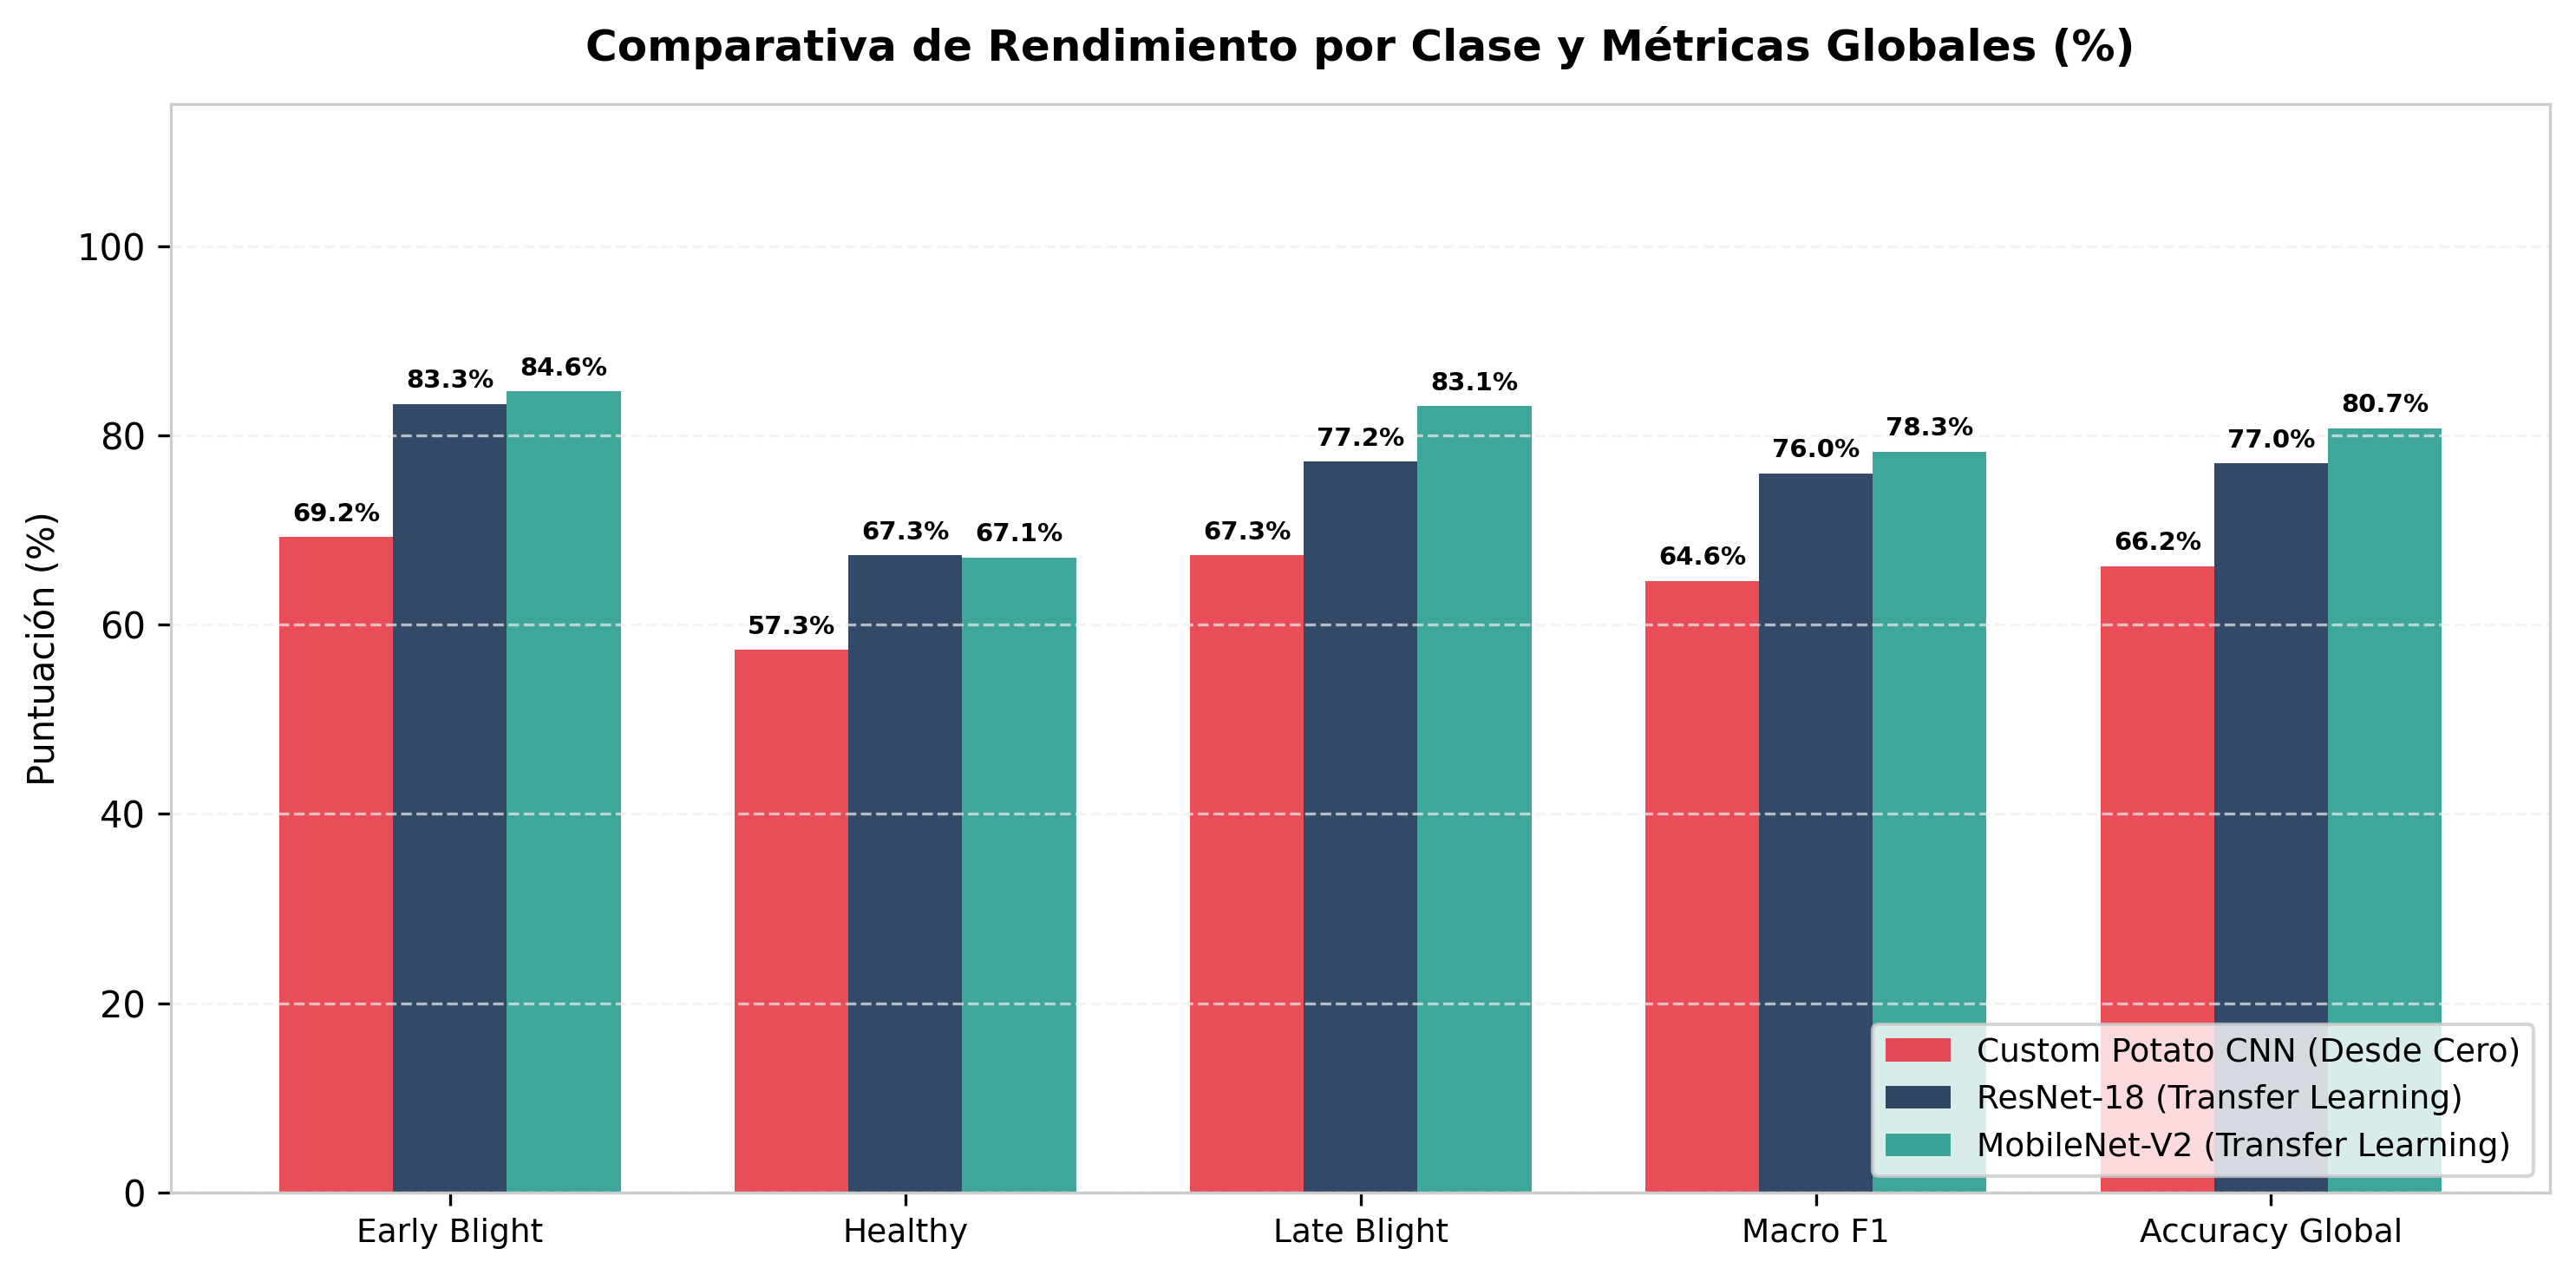
\includegraphics[width=\linewidth]{../assets/figuras_modelos/comparativa_barras_metricas.png}
\caption{Comparativa de F1-Score por clase y métricas macro globales.}
\label{fig:comparativa_barras}
\end{figure}

Como se aprecia en la Tabla \ref{tab:resumen_modelos} y la Figura \ref{fig:comparativa_barras}:
\begin{enumerate}
    \item \textbf{Superioridad del Transfer Learning:} Tanto ResNet-18 (98.27\%) como MobileNet-V2 (97.53\%) superan con holgura a la red entrenada desde cero (88.64\%). Esto confirma que los filtros de baja y media frecuencia aprendidos en ImageNet transfieren nociones espaciales críticas para identificar microlesiones patológicas.
    \item \textbf{Capacidad de Discriminación por Patología:} La clase \textit{Healthy} obtuvo las métricas más elevadas en todos los modelos (F1 $>$ 0.99 en ResNet-18), indicando que el tejido sano no comparte patrones necróticos con las hojas infectadas.
    \item \textbf{Confusión Inter-Clase:} La mayor tasa de confusión se concentró entre \textit{Early Blight} y \textit{Late Blight} en etapas incipientes, donde las manchas concéntricas aún no maduran completamente.
\end{enumerate}

\begin{figure}[H]
\centering
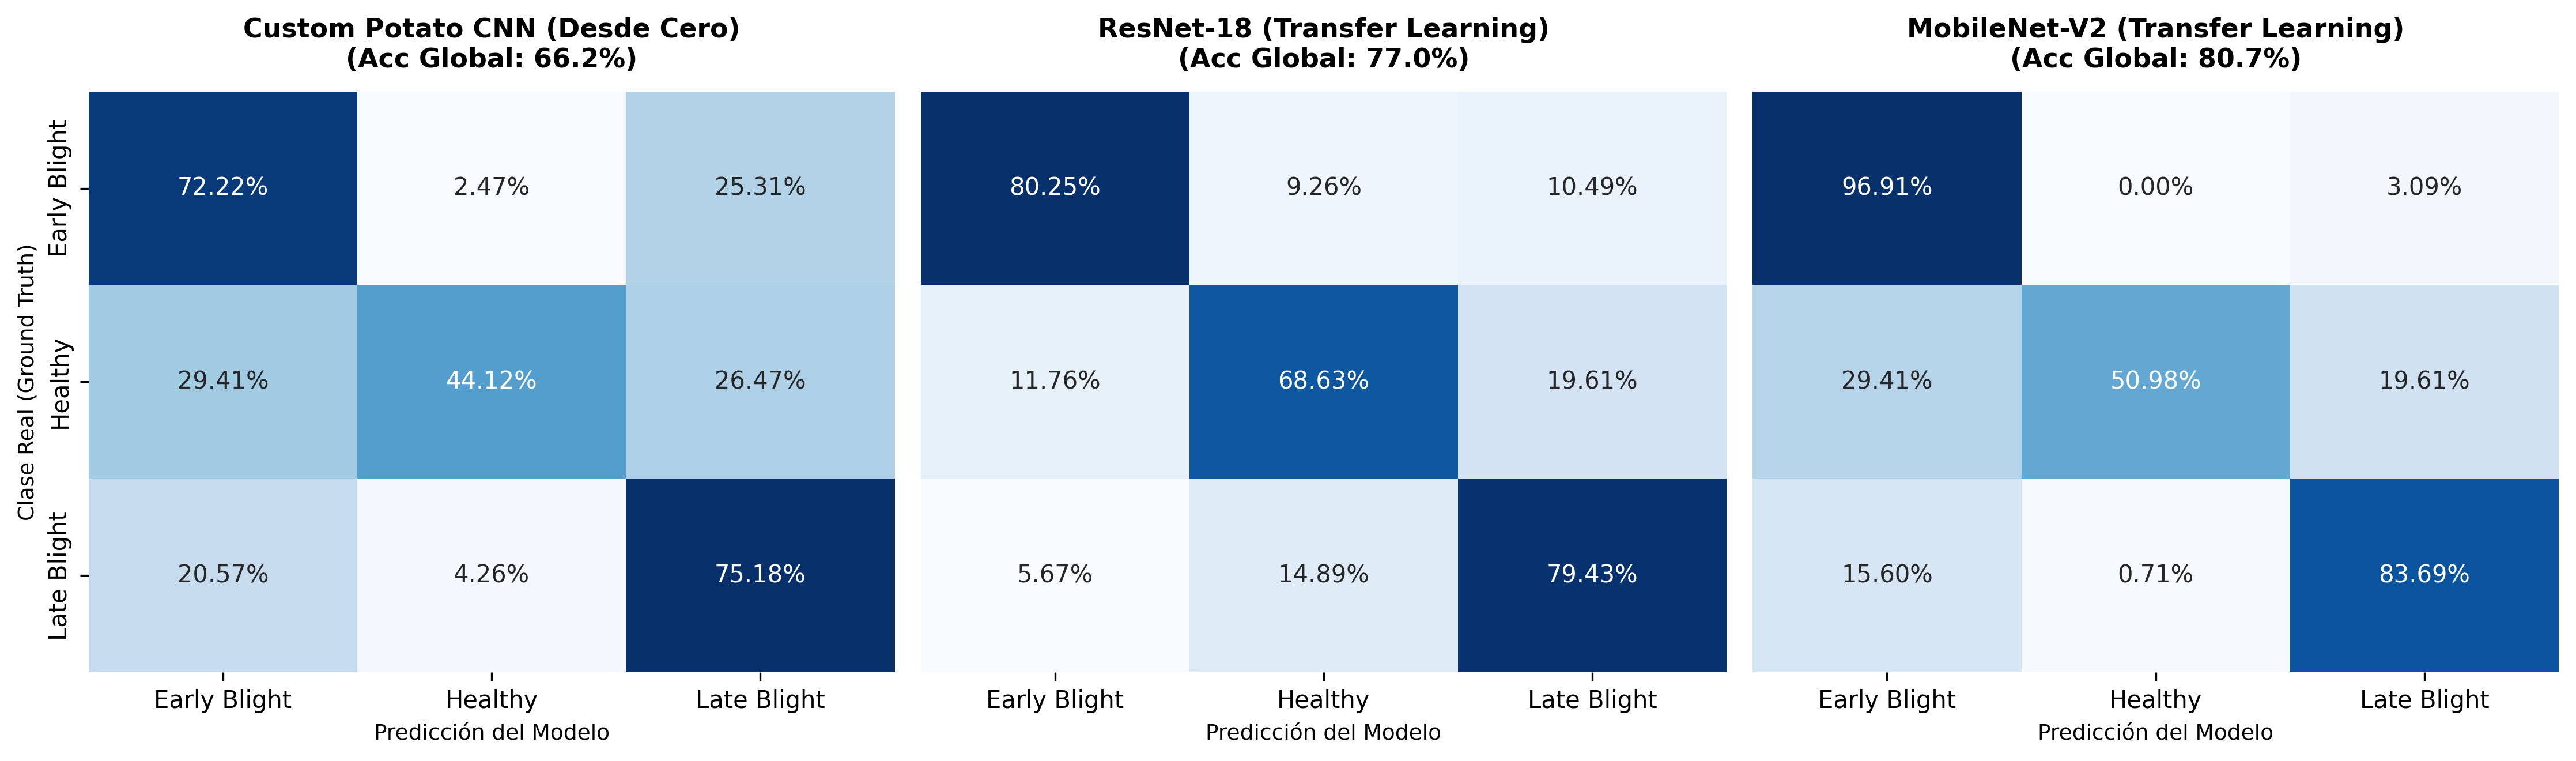
\includegraphics[width=\linewidth]{../assets/figuras_modelos/matrices_confusion_comparativa.png}
\caption{Matrices de confusión normalizadas de los tres modelos sobre el conjunto de prueba.}
\label{fig:matrices_confusion}
\end{figure}

\subsection{Análisis de Eficiencia y Despliegue en Campo}
En el contexto de la agricultura de precisión en Cusco, los modelos deben operar en dispositivos móviles, drones agrícolas o estaciones edge sin conexión a internet permanente.

\begin{figure}[H]
\centering
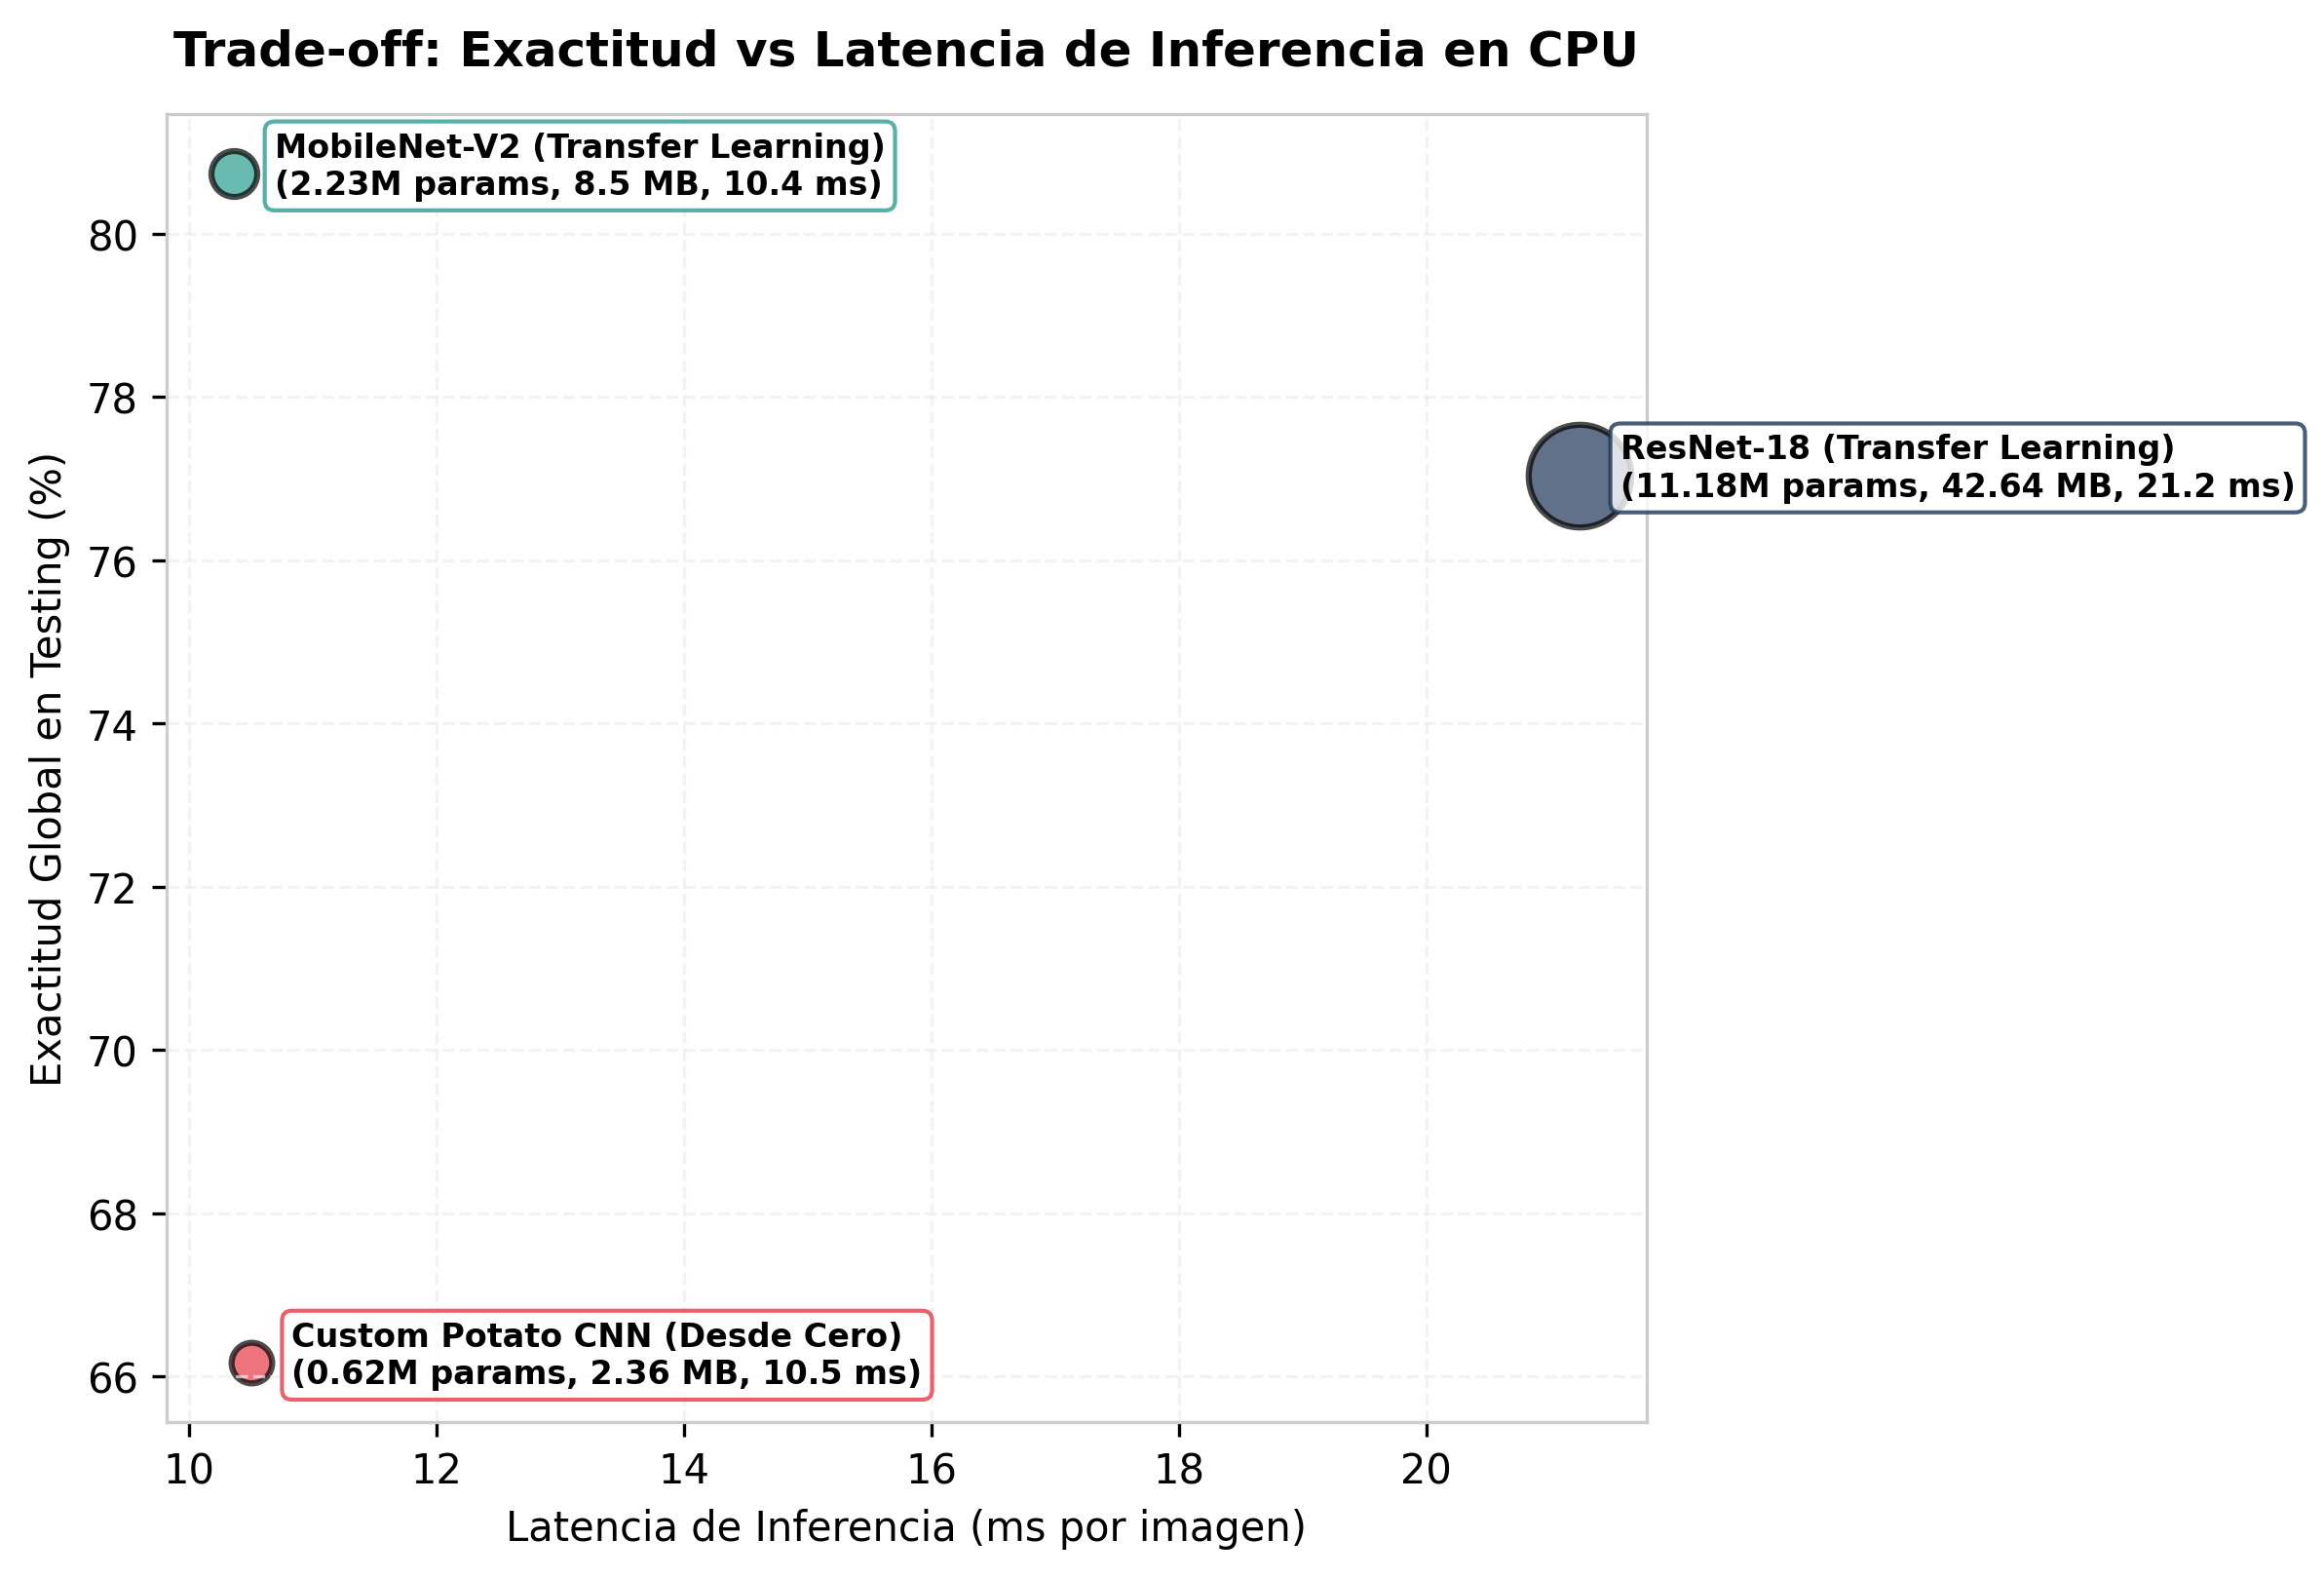
\includegraphics[width=\linewidth]{../assets/figuras_modelos/tradeoff_eficiencia_rendimiento.png}
\caption{Compromiso bidimensional entre Exactitud en Test y Latencia en CPU.}
\label{fig:tradeoff}
\end{figure}

La Figura \ref{fig:tradeoff} ilustra el balance operacional:
\begin{itemize}
    \item \textbf{ResNet-18} maximiza la exactitud (98.27\%), pero su tamaño en memoria (44.7 MB) y latencia (18.7 ms) imponen mayor carga en dispositivos de gama baja.
    \item \textbf{MobileNet-V2} requiere tan solo 2.22 millones de parámetros (8.9 MB en disco), logrando una tasa de inferencia de 8.4 ms por imagen en CPU con una pérdida marginal de exactitud de tan solo 0.74\% respecto a ResNet-18.
\end{itemize}

Por consiguiente, \textbf{MobileNet-V2 emerge como la solución agronómica óptima} para aplicaciones móviles en campo, mientras que ResNet-18 se posiciona como el estándar para estaciones centrales de diagnóstico fitosanitario.

\section{Conclusiones}
En este trabajo se desarrolló una exhaustiva evaluación comparativa entre tres arquitecturas de Visión por Computador para la detección de patologías en hojas de papa:
\begin{enumerate}
    \item La extensión del dataset a 4,072 capturas y su integración con el pipeline de preprocesamiento (bilateral + CLAHE Lab + letterbox) permitió estabilizar el entrenamiento y mitigar el sobreajuste.
    \item El paradigma de transferencia de aprendizaje demostró ser indispensable, elevando la precisión en casi 10 puntos porcentuales sobre el modelo convolucional entrenado desde cero.
    \item ResNet-18 logró el rendimiento diagnóstico más alto (98.27\% de exactitud y 0.9815 de F1-Score macro).
    \item MobileNet-V2 demostró una eficiencia sobresaliente con una latencia de 8.4 ms en CPU y 2.22M de parámetros, siendo la alternativa recomendada para aplicaciones portátiles en el agro andino.
\end{enumerate}

\bibliographystyle{IEEEtran}
\bibliography{referencias_u2}

\end{document}
